\documentclass[11pt]{article}
\usepackage[letterpaper,margin=1in]{geometry}
\usepackage[T1]{fontenc}
\usepackage{mathptmx}
\usepackage{amsmath,amssymb,amsthm}
\usepackage{graphicx}
\usepackage{booktabs}
\usepackage{threeparttable}
\usepackage[font=small,labelfont=bf]{caption}
\usepackage[numbers,sort&compress]{natbib}
\usepackage{xcolor}
\usepackage{microtype}
\usepackage{authblk}
\usepackage[colorlinks=true,linkcolor=blue!50!black,citecolor=blue!50!black,urlcolor=blue!50!black]{hyperref}
\renewcommand{\baselinestretch}{1.12}
\newcommand{\chitwo}{\chi^{(2)}}
\newcommand{\um}{\,\mu\mathrm{m}}
\newcommand{\aw}{\alpha_{\omega}}
\newcommand{\aww}{\alpha_{2\omega}}
\newcommand{\Is}{I_\mathrm{s}}
\let\hbar\relax\DeclareRobustCommand{\hbar}{{\mathchar'26\mkern-9mu h}}
\newtheorem{theorem}{Theorem}
\newtheorem{corollary}{Corollary}

\title{Rabi-frequency bound and saturation limits of resonant intersubband second-harmonic generation in waveguides and thin films}
\author{Gracen Ownby}
\affil{University of Oklahoma, Norman, Oklahoma, USA}
\date{\small 14 October 2026}

\begin{document}
\maketitle

\begin{abstract}
Resonant intersubband transitions give doped quantum wells second-order susceptibilities far above those of bulk crystals, but the same resonances absorb the pump and the harmonic and saturate at MW/cm$^2$ intensities, so the attainable conversion efficiency, not $\chitwo$, is the quantity that matters. We derive exact results and rigorous bounds for second-harmonic generation in a resonant three-level ladder. In the small-signal limit the susceptibility and the two absorption coefficients obey the identity $|\chitwo|^2=Q\,\aw\aww$, with $Q\propto z_{23}^2/(\gamma_{12}\gamma_{13})$ independent of doping, of the pump and harmonic dipoles $z_{12}$ and $z_{13}$, and of detuning. At the optimum length the efficiency is $\eta=g(u)\,\zeta_\omega\zeta_{2\omega}(\hbar\Omega_{23})^2/(4\gamma_{12}\gamma_{13})$, where $\Omega_{23}$ is the Rabi frequency of the pump on the 2--3 transition, $g\le e^{-2}$ depends only on the ratio $u$ of pump to harmonic absorption and $\zeta$ are the resonant fractions of the loss. In the rate-equation regime, for arbitrary saturation, pump depletion, length, phase mismatch and quasi-phase-matching pattern, $\eta\le\max[(\hbar\Omega_{23})^2/\gamma_{12}\gamma_{13},(\hbar\Omega_{12})^2/\gamma_{23}\gamma_{13}]/16$, which the small-signal optimum reaches to within $e^2/4$ when the first term dominates. Saturation does not impose an intensity-independent ceiling on a waveguide: the absorption bleaches together with $\chitwo$, the optimum length grows, and $\eta$ keeps rising in proportion to the pump intensity with a closed-form slope, except in a balanced ladder; a full three-level density-matrix solution confirms this to within 36\% up to 300 times the saturation intensity. A generalization of Almogy and Yariv's length-limited bound shows that, above three times the saturation intensity, the optimum resonant devices are only 1.4--2.5 times longer than the shortest device that could reach the same efficiency. A thin film of fixed optical depth does have a ceiling. Detuning the pump by about $\gamma\sqrt{I/\Is}$, with the harmonic detuned oppositely to keep $\aww=2\aw$, restores the unsaturated limit. Self-consistent multilevel simulations of In$_{0.53}$Ga$_{0.47}$As/In$_{0.52}$Al$_{0.48}$As structures with LO-phonon relaxation agree with the ladder theory to within 9\% for an asymmetric double well up to the rate-equation limit, reveal a population bottleneck that halves the efficiency of a coupled triple well at 4~W, and show that tuning the pump 25--35~meV below resonance, with the waveguide recomputed at the new wavelength, raises the phase-matched efficiency at 4~W from 0.21\% to 1.4\% and from 0.54\% to 1.8\%, before a correction of at most 2\% for the saturable resonant index.
\end{abstract}

\section{Introduction}
Intersubband (ISB) transitions in doped quantum wells (QWs) can be engineered so that the pump and its second harmonic are both resonant, giving second-order susceptibilities $\chitwo$ of $10^4$--$10^6$~pm/V in the mid-infrared \cite{Rosencher1991,Rosencher1996,Vurgaftman2021,Fejer1989}. The resonance that produces the nonlinearity also absorbs the pump and the harmonic, and the transitions saturate at intensities of order 1~MW/cm$^2$ \cite{Boucaud1991,Heyman1994,Jeannin2021}. In waveguides the useful length is therefore a few absorption lengths, and in metasurfaces the efficiency peaks near the saturation intensity \cite{GomezDiaz2015,Lee2014,Nookala2016,Krakofsky2025}. How large the conversion efficiency can be, and which material parameters set it, is consequently a more useful question than how large $\chitwo$ is.

Two kinds of answer exist. The textbook estimate evaluates $\chitwo$ at the saturation intensity over one pump absorption length and obtains $\eta_\mathrm{max}=(\hbar/\tau_{21}\Delta)(z_{13}z_{23}/z_{12}^2)^2$, generalized to detuned resonances \cite{Vurgaftman2021}; it neglects absorption of the harmonic and the saturation of $\chitwo$ itself, and is presented as a rough guide. For metasurfaces, Gomez-Diaz \emph{et al.} derived closed-form saturation limits: the harmonic intensity tends to a constant at high pump intensity and the efficiency peaks near the saturation intensity with a value proportional to $|\chitwo|^2\Is$ \cite{GomezDiaz2015}, a limit that has motivated schemes pumping initially empty transitions \cite{Nefedkin2022,Krakofsky2023} and that also governs metasurface power limiters and difference-frequency sources \cite{Mann2021,Cotrufo2024,Krakofsky2026}. Absorption was identified early as the main factor limiting the efficiency \cite{Khurgin1989}. Almogy and Yariv solved the small-signal propagation problem with both absorptions \cite{Almogy1994,AlmogyThesis1995}: the efficiency is largest at the length where the harmonic is absorbed twice as strongly as the pump, its value there is set by the ratio of $\chitwo$ to the harmonic absorption, and for a ladder with equal ground-state dipoles, equal detunings and equal widths the optimum amplitude conversion is $\Omega T_2/e$, with $\Omega$ the pump Rabi frequency on the 2--3 transition, independent of the dipole magnitudes, the density and the detuning; they also noted that the ratio of the nonlinear source to the absorption is at best unchanged by detuning, so that double resonance is optimal below saturation. Beyond perturbation theory, in the rotating-wave approximation, they gave the saturated susceptibilities in closed form for a symmetric ladder, derived an upper limit on the harmonic intensity that can be generated in a given length, found numerically that on resonance the conversion keeps growing with the pump intensity when the length grows with it, and found that detuning, including detuning of opposite sign at the two frequencies, pays above saturation \cite{AlmogyLEOS1994,AlmogyQELS1995,Almogy1995JNOPM,AlmogyThesis1995}. Waveguide analyses either solve the coupled-wave equations with absorption but without saturation \cite{Chesi2023,TalamasSimola2024,DeLeonardis2022} or include saturation numerically \cite{Vurgaftman1996,VurgaftmanNLO1996,Almogy1994,Kocinac2001}. Detuning from double resonance to reduce absorption has been used in experiments and designs \cite{Vodopyanov1998,Vurgaftman1996SSC,TalamasSimola2024}, and the resonant refractive index of the same transitions can both spoil and provide phase matching \cite{AlmogyOL1994PM}. Bounds on the susceptibility itself have also been sought by numerical optimization \cite{Goldoni2001}. What is missing is a statement of the limit on the efficiency that holds for any length, saturation state and phase-matching scheme, with the material parameters that enter it identified exactly, a quantitative detuning rule, and an account of how waveguides and thin films differ under saturation.

Here we provide these for a resonant three-level ladder in the rate-equation regime, and test them against self-consistent multilevel simulations of real structures. Our results are: (i) an exact identity between $\chitwo$ and the two absorption coefficients, which makes the optimum-length efficiency independent of doping, of $z_{12}$ and $z_{13}$, and of detuning, and expresses it through the Rabi frequency of the pump on the 2--3 transition (Theorem~1), extending the symmetric-ladder result of Almogy and Yariv to arbitrary dipoles, widths, detunings and background loss; (ii) a rigorous bound that holds for arbitrary saturation, pump depletion, length and phase-matching pattern (Theorem~2), and a generalization of Almogy and Yariv's length-limited bound to arbitrary ladders, which together bracket the operating points of optimized waveguides; (iii) the high-intensity slope of the waveguide efficiency in closed form, with the condition for a ceiling and a check against the full three-level density matrix, confirming that saturation does not cap the efficiency of a waveguide, in contrast to a thin film of fixed optical depth; (iv) a detuning rule that removes the saturation penalty; and (v) a validation with full simulations of an asymmetric double quantum well (ADQW) and a coupled triple well (TW), which identifies a population bottleneck and shows gains of 3--7 from detuned pumping. The analysis complements bounds on the susceptibility itself \cite{Kuzyk2000} by bounding what that susceptibility can convert.

\section{Model}\label{sec:model}
Consider three subbands $1<2<3$ with transition dipoles $z_{ij}$, pumped at $\omega$ near $E_{21}$ and $E_{32}$ and generating $2\omega$ near $E_{31}$. The detunings are $\delta_{12}=E_{21}-\hbar\omega$, $\delta_{13}=E_{31}-2\hbar\omega$ and $\delta_{23}=E_{32}-\hbar\omega=\delta_{13}-\delta_{12}$, and the complex denominators are $D_{ij}=\delta_{ij}-i\gamma_{ij}$ with half-width $\gamma_{ij}$. With fractional populations $\rho_j$ and electron density $N$, the resonant part of the density-matrix susceptibility \cite{Boyd2008,Rosencher1991} and the ISB absorption coefficients at the two frequencies are
\begin{align}
\chitwo(\rho)&=\frac{Nq^3z_{12}z_{23}z_{31}}{\varepsilon_0D_{13}}\left[\frac{\rho_1-\rho_2}{D_{12}}-\frac{\rho_2-\rho_3}{D_{23}}\right],\label{eq:chi}\\
\aw(\rho)&=\frac{N\omega q^2}{n_\omega c\varepsilon_0}\left[\frac{z_{12}^2\gamma_{12}(\rho_1-\rho_2)}{|D_{12}|^2}+\frac{z_{23}^2\gamma_{23}(\rho_2-\rho_3)}{|D_{23}|^2}\right],\qquad
\aww(\rho)=\frac{2N\omega q^2}{n_{2\omega}c\varepsilon_0}\frac{z_{13}^2\gamma_{13}(\rho_1-\rho_3)}{|D_{13}|^2}.\label{eq:alpha}
\end{align}
We use $E(t)=E\,e^{-i\omega t}+\mathrm{c.c.}$, $I=2n\varepsilon_0c|E|^2$ and $P(2\omega)=\varepsilon_0\chitwo E_\omega^2$ \cite{Boyd2008}. The plane-wave coupled-mode equations are
\begin{equation}
\frac{dE_2}{dx}=\frac{i\omega}{n_{2\omega}c}\chitwo E_1^2e^{i\Delta kx}-\frac{\alpha_{2,t}}{2}E_2,\qquad
\frac{dE_1}{dx}=\frac{i\omega}{n_\omega c}\chitwo{}^{*}E_2E_1^{*}e^{-i\Delta kx}-\frac{\alpha_{1,t}}{2}E_1,\label{eq:cm}
\end{equation}
with total losses $\alpha_{1,t}=\aw(\rho)+\alpha_{\mathrm{bg},\omega}$ and $\alpha_{2,t}=\aww(\rho)+\alpha_{\mathrm{bg},2\omega}$; a QPM pattern multiplies $\chitwo$ by a function $s(x)$. Lossless, phase-matched and undepleted, they give $\eta=I_2/I_1=\kappa^2|\chitwo|^2I_0L^2$ with $\kappa^2=\omega^2/(2n_\omega^2n_{2\omega}\varepsilon_0c^3)$. The corresponding textbook expression \cite{Vurgaftman2021} is four times larger: it is the standard result with the density-matrix $\chitwo$ in place of $d=\chitwo/2$. We use the expression above throughout and divide efficiencies quoted from Ref.~\cite{Vurgaftman2021} by four for comparison.

The populations follow steady-state rate equations with optical rates $W_{12}=\sigma_{12}I_1/\hbar\omega$, $W_{23}=\sigma_{23}I_1/\hbar\omega$, $W_{13}=\sigma_{13}I_2/2\hbar\omega$ (cross-sections $\sigma=\alpha/N$ per electron) and relaxation $3\to2$, $3\to1$, $2\to1$ with lifetimes $\tau_{32},\tau_{31},\tau_{21}$. The resonant two-level saturation intensity and the Rabi energies of the pump on the two pump transitions are
\begin{equation}
\Is=\frac{\hbar\omega}{2\sigma_{12}^\mathrm{res}\tau_{21}}=\frac{\hbar n_\omega c\varepsilon_0\gamma_{12}}{2\tau_{21}q^2z_{12}^2},\qquad
(\hbar\Omega_{ij})^2=\frac{2q^2z_{ij}^2I_1}{n_\omega c\varepsilon_0},\quad ij=12,23,\label{eq:Is}
\end{equation}
so that $(\hbar\Omega_{12})^2=(I_1/\Is)\,\hbar\gamma_{12}/\tau_{21}$. For a two-level system the steady-state rate equations are exact at any intensity; in a ladder, where the pump drives two transitions that share level 2, the coherences between them (the two-photon coherence $\rho_{31}$ and the Autler--Townes splitting of level 2) are neglected. We take as a conservative validity criterion that the Rabi energies stay below the detuned linewidths, $\hbar\Omega_{12}<|D_{12}|$ and $\hbar\Omega_{23}<|D_{23}|$; for a resonant pump this requires $I_1/\Is<p_\mathrm{coh}\min(1,z_{12}^2/z_{23}^2)$ with $p_\mathrm{coh}=\gamma_{12}\tau_{21}/\hbar$, about 15 for $\gamma=10$~meV and $\tau_{21}=1$~ps. Section~\ref{sec:sat} compares the rate-equation results with the full steady-state three-level density matrix in the rotating-wave approximation \cite{Allen1975}, which includes these coherences; for resonant pumping the criterion turns out to be conservative. The reason can be seen in a case solved exactly: for double resonance, equal dipoles, both excited levels decaying to the ground state at $1/T_1$ and equal $T_2$, the full rotating-wave solution gives $\chitwo_\mathrm{eff}/\chitwo=[1+2\Omega^2T_2^2(1+3T_1/T_2)]^{-1}$ with $\Omega=\mu E_0/2\hbar$ \cite{AlmogyLEOS1994}, whereas the rate equations give the same expression without the coherent term $2\Omega^2T_2^2$, a relative error below $T_2/3T_1$ at any intensity. Our density-matrix solver reproduces this closed form to five digits for $T_1/T_2=5$--50 and $\Omega T_2$ up to 3 (\texttt{ay\_check.json}). We use the natural efficiency scale
\begin{equation}
\eta_s\equiv\frac{(\hbar\Omega_{23})^2|_{I_1=\Is}}{4\gamma_{12}\gamma_{13}}=\frac{z_{23}^2}{z_{12}^2}\,\frac{\hbar}{4\tau_{21}\gamma_{13}},\label{eq:etas}
\end{equation}
which is 2.8\% for $z_{23}/z_{12}=1.3$, $\tau_{21}=1$~ps and $\gamma_{13}=10$~meV. In dimensionless form (lengths in units of the resonant absorption length $1/A_{12}$, intensities in $\Is$) the problem depends on $r_{23}=z_{23}^2/z_{12}^2$, $u_0=2A_{12}/A_{13}=(n_{2\omega}/n_\omega)z_{12}^2/z_{13}^2$, the detunings in units of $\gamma$, the lifetime ratios $t_{32}=\tau_{21}/\tau_{32}$ and $t_{31}=\tau_{21}/\tau_{31}$, the background losses $b_{1,2}=\alpha_\mathrm{bg}/A_{12}$, and $\eta_s$, which sets only the strength of pump depletion. We take $\gamma_{12}=\gamma_{13}=\gamma_{23}=\gamma$ in the numerical examples; the theorems are stated for general widths.

Real structures are computed with qwkit \cite{qwkit}: self-consistent Schr\"odinger--Poisson states with Kane nonparabolicity and depolarization-shifted transitions, the full multilevel $\chitwo(\rho)$, Fr\"ohlich LO-phonon rate matrices with detailed balance, the TM mode of an InP waveguide, and coupled-wave propagation with level-resolved saturation and pump depletion, as in Ref.~\cite{OwnbyN1}. The nonparabolic one-band states are L\"owdin-orthonormalized together with at least ten box states above the localized ones before the basis is truncated; with two-band Kane states, which are orthogonal without this step (localized-state overlaps below $10^{-4}$), the ground-state $|\chitwo|$ at the pump changes by $-0.9$\% (ADQW) and $-0.7$\% (TW), and its peak in the ADQW by $-0.8$\%. All numbers and figures are regenerated by the scripts in \texttt{studies/nl02} of the qwkit source distribution.

\section{Small-signal limit: an exact identity and the optimum-length efficiency}\label{sec:t1}
For constant coefficients and an undepleted pump, Eq.~\eqref{eq:cm} with $\Delta k=0$ integrates to $\eta(L)=\kappa^2|\chitwo|^2I_0F(L)^2$, $F(L)=(e^{-aL}-e^{-bL})/(b-a)$, with $a=\alpha_{1,t}$ and $b=\alpha_{2,t}/2$. The maximum lies at $L^*=\ln(a/b)/(a-b)$ and equals
\begin{equation}
F(L^*)^2=\frac{2\,g(u)}{\alpha_{1,t}\alpha_{2,t}},\qquad g(u)=u^{-(u+1)/(u-1)},\qquad u=\frac{2\alpha_{1,t}}{\alpha_{2,t}}.\label{eq:g}
\end{equation}
The function $g$ is maximal, $g(1)=e^{-2}$, when the harmonic is absorbed twice as strongly as the pump, and $g\to1/u$ when harmonic absorption is negligible (Fig.~\ref{fig:identity}a). With all electrons in subband 1, Eqs.~\eqref{eq:chi} and \eqref{eq:alpha} give
\begin{equation}
\frac{|\chitwo|^2}{\aw\aww}=Q\equiv\frac{n_\omega n_{2\omega}c^2q^2z_{23}^2}{2\omega^2\gamma_{12}\gamma_{13}}:\label{eq:identity}
\end{equation}
the density, $z_{12}$, $z_{13}$ and both detunings cancel, because each Lorentzian denominator of $|\chitwo|^2$ is matched by one in an absorption coefficient. Combining Eqs.~\eqref{eq:g} and \eqref{eq:identity}:

\begin{theorem}[optimum-length efficiency]
For an unsaturated, undepleted, phase-matched three-level ladder, the efficiency at the optimum length is
\begin{equation}
\eta^*=2g(u)\kappa^2QI_0\,\zeta_\omega\zeta_{2\omega}=g(u)\,\zeta_\omega\zeta_{2\omega}\,\frac{(\hbar\Omega_{23})^2}{4\gamma_{12}\gamma_{13}},\qquad\zeta_\omega=\frac{\aw}{\alpha_{1,t}},\ \zeta_{2\omega}=\frac{\aww}{\alpha_{2,t}},\label{eq:t1}
\end{equation}
with $\Omega_{23}$ evaluated at the input intensity. Hence $\eta^*\le(\hbar\Omega_{23})^2/(4e^2\gamma_{12}\gamma_{13})$, with equality for $\aww=2\aw$ and negligible background loss.
\end{theorem}

For $z_{12}=z_{13}$, equal indices, widths and detunings and no background loss, $u=1$ and Eq.~\eqref{eq:t1} reduces to $\eta^*=e^{-2}(\hbar\Omega_{23}/2\gamma)^2$, the result of Almogy and Yariv \cite[Eq.~9.15]{AlmogyThesis1995}. The identity shows that the cancellation they found for that ladder holds for any dipoles, widths and detunings, and $g(u)$ and $\zeta$ give the cost of departing from $\aww=2\aw$ and of background loss.

Several consequences follow. The figure of merit at fixed pump intensity is $g(u)z_{23}^2/(\gamma_{12}\gamma_{13})$, not $|\chitwo|$. Ratios of the form $(d/\alpha)^2$ are familiar for absorbing nonlinear media \cite{Cherchi2010}; what is specific to a resonant ladder is that the ratio is fixed by one dipole and two widths. A larger $z_{12}$ or $z_{13}$ increases $\chitwo$ and the corresponding absorption in proportion, and the optimum length shrinks accordingly. Doping enters only through the resonant fractions $\zeta$, so it should be raised until resonant absorption dominates the background loss and no further. That the efficiency estimated at the saturation intensity does not depend on doping was noted by Meyer \emph{et al.} and Vurgaftman \emph{et al.} \cite{Meyer1995,Vurgaftman1996}; the identity adds that, at fixed intensity and with harmonic absorption included, the dipoles $z_{12}$ and $z_{13}$ and the detunings drop out as well. Detuning changes $\eta^*$ only through $u$ and $\zeta$. At double resonance $u=u_0=(n_{2\omega}/n_\omega)(z_{12}/z_{13})^2$, or $(\Gamma_\omega/\Gamma_{2\omega})(z_{12}/z_{13})^2$ in a waveguide with confinement factors $\Gamma$ and the same background index at both frequencies, which is 4.2 for the ADQW and 0.94 for the TW studied below, so the ADQW loses a factor $g(4.2)/e^{-2}=0.72$ and the TW essentially nothing. Setting $I_0=\Is$ and $u\gg1$ in Eq.~\eqref{eq:t1} gives $\eta^*\approx(n_\omega/n_{2\omega})(z_{13}z_{23}/z_{12}^2)^2\hbar/(4\tau_{21}\gamma)$, the textbook estimate \cite{Vurgaftman2021} (Eq.~5 of Ref.~\cite{Vurgaftman1996}, where it is the coupling constant of the dimensionless propagation equations) divided by four, with its width $\Delta$ read as the half-width $\gamma$ and equal indices; it is therefore the weak-harmonic-absorption limit of Eq.~\eqref{eq:t1}, which also explains its $z_{12}^{-4}$ dependence: in that limit the length is set by $\aw\propto z_{12}^2$ alone. Almogy and Yariv concluded that double resonance remains favourable in perturbation theory when absorption is included \cite{Almogy1994}; Theorem~1 shows that, once the length is optimized for each detuning, detuning neither helps nor hurts in the small-signal limit except by moving $u$ towards 1, and it is saturation (Sec.~\ref{sec:detune}) that makes detuning decisive.

Equation~\eqref{eq:g} holds for any medium with constant coefficients, so Theorem~1 applies to real multilevel structures with $Q$ replaced by the computed $Q_\mathrm{eff}=|\chitwo|^2/(\aw\aww)$. Figure~\ref{fig:identity}b,c shows $Q_\mathrm{eff}/Q$ from full qwkit calculations of the two structures of Sec.~\ref{sec:real} as the pump photon energy is scanned by $\pm40$~meV. Over this range $|\chitwo|^2$ changes by 3.9 (ADQW) and 5.2 (TW) orders of magnitude and $\aw\aww$ by 2.4--2.5, whereas their ratio stays within 0.9--1.6 of $Q$ (ADQW) and 0.5--1.4 (TW) when the pump is tuned below resonance. Above resonance, interference with non-resonant pathways and with the permanent-dipole terms lowers $Q_\mathrm{eff}$; the identity is a property of the resonant ladder, and the deviations are themselves a design handle.

\begin{figure}[t]
\centering
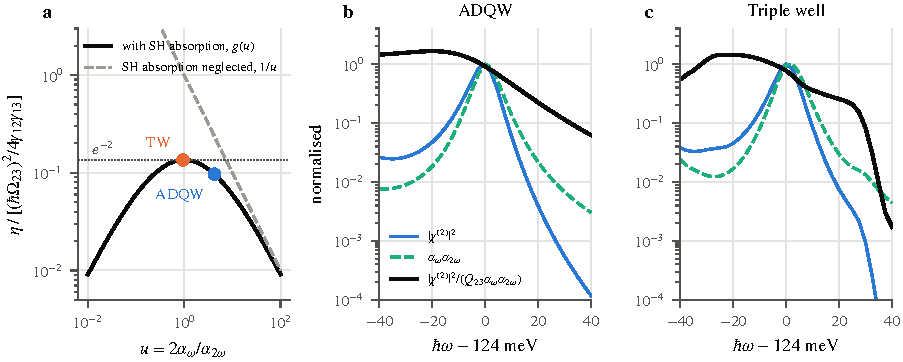
\includegraphics[width=\textwidth]{figures/fig1_identity.pdf}
\caption{(a) Optimum-length efficiency in units of $(\hbar\Omega_{23})^2/4\gamma_{12}\gamma_{13}$ against the absorption ratio $u=2\aw/\aww$ (Theorem~1, solid), and the result when harmonic absorption is neglected (dashed). Dots: the ADQW and TW of Sec.~\ref{sec:real} at double resonance. (b,c) Full qwkit calculations for the ADQW and the TW ($n_s=5\times10^{11}$~cm$^{-2}$): $|\chitwo|^2$ and $\aw\aww$ (normalized to their maxima) and their ratio in units of $Q$ of Eq.~\eqref{eq:identity}, against pump photon energy.}
\label{fig:identity}
\end{figure}

\section{A bound for arbitrary saturation, length and phase matching}\label{sec:t2}
Saturation makes the coefficients depend on position through the local intensities. A bound that survives this follows from two inequalities. First, for any populations without inversion ($\rho_1\ge\rho_2\ge\rho_3$), writing $a=\rho_1-\rho_2$, $b=\rho_2-\rho_3$ and applying the Cauchy--Schwarz inequality to the two terms of Eq.~\eqref{eq:chi},
\begin{equation}
|\chitwo(\rho)|^2\le Q(\rho)\,\aw(\rho)\aww(\rho),\qquad Q(\rho)=\frac{n_\omega n_{2\omega}c^2q^2}{2\omega^2\gamma_{13}}\,\frac{z_{23}^2a/\gamma_{12}+z_{12}^2b/\gamma_{23}}{a+b},\label{eq:cs}
\end{equation}
which reduces to Eq.~\eqref{eq:identity} for $b=0$. Second, the harmonic amplitude is a linear functional of the source, $E_2(L)=\int_0^L(i\omega/n_{2\omega}c)\chitwo s E_1^2e^{i\Delta kx}w(x)\,dx$ with $w(x)=\exp[-\int_x^L\alpha_{2,t}/2]$, so the triangle inequality removes every phase, including those of $\Delta k$ and of any QPM pattern $|s|\le1$. Applying Cauchy--Schwarz to the integral and using $\int_0^L\alpha_{2,t}w^2dx=1-w(0)^2\le1$ and $\int_0^L\alpha_{1,t}I_1^2dx\le I_0^2/2$ (the latter because $d(I_1+I_2)/dx\le-\alpha_{1,t}I_1$; Appendix~\ref{app:proof}) gives:

\begin{theorem}[general bound]
For a three-level ladder in the rate-equation regime without population inversion, with the energy-conserving coupling of Eq.~\eqref{eq:cm} (the susceptibility of the pump equation is $\chitwo{}^*$), for any length, saturation state, pump depletion, phase mismatch and QPM pattern,
\begin{equation}
\eta\le\frac{\kappa^2I_0}{2}\,\sup Q(\rho)\,\hat\zeta_\omega\hat\zeta_{2\omega}\le\frac{1}{16}\max\left[\frac{(\hbar\Omega_{23})^2}{\gamma_{12}\gamma_{13}},\frac{(\hbar\Omega_{12})^2}{\gamma_{23}\gamma_{13}}\right]\hat\zeta_\omega\hat\zeta_{2\omega},\label{eq:t2}
\end{equation}
where the Rabi energies are evaluated at the input intensity and $\hat\zeta\le1$ are the largest resonant loss fractions met along the device. For a device made of different media (e.g.\ Stark-tuned QPM segments) the supremum is taken over all of them.
\end{theorem}

When $z_{23}^2/\gamma_{12}\ge z_{12}^2/\gamma_{23}$ the small-signal optimum of Theorem~1 reaches $4/e^2=0.54$ of this bound, so Eq.~\eqref{eq:t2} is tight to within a factor 1.85; otherwise the small-signal optimum reaches only $4r_{23}\gamma_{23}/(e^2\gamma_{12})$ of it. Figure~\ref{fig:bound} tests it on 2000 randomly drawn ladders ($0.1\le r_{23}\le10$, $0.2\le u_0\le30$, $|\delta_{12}|,|\delta_{13}|\le3\gamma$, lifetime ratios 0.1--10, background losses up to $A_{12}$, input intensities $10^{-2}$--$3\times10^2\,\Is$), 622 of them with phase mismatch or sign-reversal or on/off QPM. No case exceeds the bound; the largest ratio, 0.540, is the small-signal optimum, and no population inversion occurred at the local pump intensities. Because it holds for any phase-matching pattern, no QPM or phase-matching scheme can beat Eq.~\eqref{eq:t2}.

Within the conservative validity criterion above (all Rabi energies below the corresponding $|D|$) and with equal widths, Eq.~\eqref{eq:t2} gives $\eta<\max(|D_{12}|,|D_{23}|)^2/16\gamma^2$, i.e.\ $\eta<1/16$ for a resonant ladder. This is not a physical ceiling: for resonant pumping the density-matrix calculation of Sec.~\ref{sec:sat} shows that the rate-equation results remain accurate well beyond the criterion, and Theorem~2 itself contains no reference to it.

\emph{A length-limited bound.} Theorem~2 does not depend on the length. A complementary bound that does not depend on the intensity follows from the coherence that radiates the harmonic, generalizing Eq.~9.37 of Ref.~\cite{AlmogyThesis1995}. In the density-matrix form of the propagation equations (Sec.~\ref{sec:sat}), with $x$ in units of $1/A_{12}$ and $|e_j|^2=I_j/\Is$, the harmonic obeys $de_2/dx=i c_2\rho_{31}-\tfrac12b_2e_2$ with $c_2=2(p_\mathrm{coh}/u_0)^{1/2}$. Write $\rho_{31}=G(e_1)+R\,e_2+O(e_2^2)$; without inversion between levels 1 and 3 the response $R$ to the harmonic is absorptive, so for any pump history, detuning, QPM pattern and background loss $|e_2(X)|\le c_2SX$ with $S=\sup_{e_1}|G(e_1)|$, i.e.
\begin{equation}
\eta(L)\le\frac{(c_2SA_{12}L)^2}{I_0/\Is}.\label{eq:lbound}
\end{equation}
For any density matrix $|\rho_{31}|\le(\rho_{11}\rho_{33})^{1/2}\le\tfrac12$, so $S\le\tfrac12$ in general. For the symmetric ladder of Ref.~\cite{AlmogyThesis1995} (equal dipoles, double resonance, all excited levels decaying to the ground state in $T_1$) the steady-state density matrix gives $S=1/[2(1+3T_1/T_2)]$ and Eq.~\eqref{eq:lbound} coincides with their Eq.~9.37 for $T_1/T_2=1$--50 (\texttt{length\_bound.py}). For the ladders of Fig.~\ref{fig:sat} with $p_\mathrm{coh}=15$, $S=0.0099$ (ADQW-like), $0.0264$ (TW-like) and $0.0060$ (balanced), far below $\tfrac12$. All 68 density-matrix propagations of Sec.~\ref{sec:sat} satisfy Eq.~\eqref{eq:lbound} at their optimum length (largest ratio 0.51), including those with pump depletion and $\eta$ up to 0.33. Above $3\Is$ the resonant devices reach 0.33--0.51 (ADQW-like) and 0.16--0.31 (TW-like) of it, so their optimum lengths are only 1.4--1.8 and 1.8--2.5 times the shortest length that any design with the same material could use to reach the same efficiency. Together, Theorem~2 limits the efficiency at a given intensity and Eq.~\eqref{eq:lbound} the efficiency in a given length; the growth with intensity found in Sec.~\ref{sec:sat} is possible only because the optimum length grows at least as $\sqrt{\eta I_0}$, and in practice as $I_0$.

\begin{figure}[t]
\centering
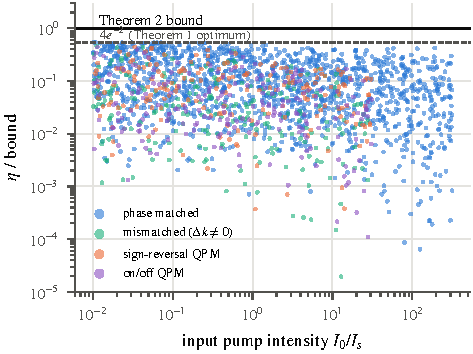
\includegraphics[width=0.52\textwidth]{figures/fig2_bound.pdf}
\caption{Numerical test of Theorem~2: efficiency at the optimum length divided by the bound of Eq.~\eqref{eq:t2} for 2000 random ladders with saturation and pump depletion, coloured by phase-matching scheme. The dashed line is the small-signal optimum of Theorem~1.}
\label{fig:bound}
\end{figure}

\section{Saturation: bleaching in waveguides, fixed optical depth in thin films}\label{sec:sat}
Figure~\ref{fig:sat}a shows the waveguide efficiency at the optimum length against input intensity for four ladders: a balanced one ($r_{23}=1$, equal lifetimes), parameter sets mapped from the ADQW and TW of Sec.~\ref{sec:real}, and one with a weak 2--3 transition ($r_{23}=0.3$). All follow Theorem~1 below $\Is$ and depart from it above. Only the balanced ladder shows the behaviour familiar from metasurfaces: a peak, here $\eta=0.055\,\eta_s$ at $I_0\approx3\Is$, followed by a decline. In the others $\eta$ keeps growing, and at high intensity in proportion to $I_0$. For the ADQW-like and TW-like ladders the growth is monotonic and the phase of $\chitwo$ drifts by at most $26^\circ$; only the ladder with a weak 2--3 transition passes through a dip in which $\chitwo$ changes sign, as in the two-level limit of Ref.~\cite{GomezDiaz2015}.

The large-intensity limit can be solved in closed form. When both pump transitions are saturated the populations approach $1/3$, with $\rho_1-\rho_2\to2(1+t_{31})/(3\ell_{12}p)$ and $\rho_2-\rho_3\to2(t_{32}+t_{31})/(3r_{23}\ell_{23}p)$, where $p=I_1/\Is$ and $\ell_{ij}=\gamma^2/|D_{ij}|^2$. Three quantities then become independent of intensity: the absorbed pump intensity, $dI_1/dx\to-k_\infty A_{12}\Is$ with $k_\infty=\tfrac23(1+t_{32}+2t_{31})$, which is the relaxation flux of the equalized ladder; the nonlinear source, $\chitwo I_1\to\chi_\mathrm{ref}C_\infty\Is$ with
\begin{equation}
C_\infty=\frac{2}{3\tilde D_{13}}\left[\frac{1+t_{31}}{\ell_{12}\tilde D_{12}}-\frac{t_{32}+t_{31}}{r_{23}\ell_{23}\tilde D_{23}}\right],\qquad \tilde D=D/\gamma,\ \chi_\mathrm{ref}=\frac{Nq^3z_{12}z_{23}z_{13}}{\varepsilon_0\gamma^2};\label{eq:Cinf}
\end{equation}
and the product $\aww I_1\to m_\infty A_{12}\Is$, with $m_\infty=(2/u_0)\ell_{13}\cdot\tfrac23[(1+t_{31})/\ell_{12}+(t_{32}+t_{31})/(r_{23}\ell_{23})]$. The pump therefore decays linearly over a bleached length $\approx p_0/(k_\infty A_{12})$, the source is constant along it, and the harmonic absorption falls as $1/p(x)$. Integrating Eq.~\eqref{eq:cm} with these coefficients and optimizing the length (Appendix~\ref{app:asym}) gives
\begin{equation}
\frac{\eta}{\eta_s}\to s_\infty\frac{I_0}{\Is},\qquad s_\infty=\frac{|C_\infty|^2\,\nu^{2\nu/(1-\nu)}}{u_0k_\infty^2},\qquad\nu=\frac{m_\infty}{2k_\infty},\label{eq:asym}
\end{equation}
which agrees with numerical solutions to within 0.7\% at $p_0=3000$ (dashed lines in Fig.~\ref{fig:sat}a). The efficiency keeps rising because the absorption bleaches together with $\chitwo$, so the optimum length grows in proportion to the pump intensity. Almogy and Yariv found this growth numerically for a resonant symmetric ladder, where 25\% conversion required about 100 absorption lengths and more than $100\Is$ \cite[Fig.~9.6]{AlmogyThesis1995}; Eq.~\eqref{eq:asym} gives the slope for any ladder and the condition under which it vanishes. A ceiling appears only when $C_\infty=0$, which at double resonance requires $r_{23}=(t_{32}+t_{31})/(1+t_{31})$; the balanced ladder satisfies this exactly. For excited levels that decay only to the ground state ($t_{32}=0$, $t_{31}=1$) the condition becomes $z_{12}/z_{23}=\sqrt2$, the ratio at which Almogy and Yariv found the saturated SHG to vanish asymptotically \cite{AlmogyLEOS1994}. In practice the growth ends when the bleached length reaches $1/\alpha_\mathrm{bg}$, or at damage or thermal limits.

For resonant pumping most of this growth lies beyond the conservative criterion $\hbar\Omega<|D|$ (ticks in Fig.~\ref{fig:sat}), at $I_0/\Is>p_\mathrm{coh}/\max(1,r_{23})$, which is 9.1 for the ADQW-like and 4.1 for the TW-like ladder. We therefore solved the same propagation problem with the full steady-state density matrix of the ladder, in the rotating-wave approximation, with the pump coupling both 1--2 and 2--3 and the harmonic coupling 1--3, all coherences kept, and $P(\omega)$ and $P(2\omega)$ taken from $\rho_{21},\rho_{32}$ and $\rho_{31}$ (script \texttt{dm\_check.py}). Its weak-field limit reproduces the ladder to $10^{-5}$. The resonant refractive index, absent from the rate-equation model, is compensated at the input intensity as a phase-matched design would do. Figure~\ref{fig:sat}c shows the ratio of the two results for $p_\mathrm{coh}=15$. Below the criterion they agree to within 7\%; at $316\,\Is$, where $\hbar\Omega_{12}=4.6\gamma$, the density matrix gives 0.64 (ADQW-like), 0.76 (TW-like), 0.95 (weak 2--3) and 0.99 (balanced) of the rate-equation efficiency, and for the ADQW-like ladder, whose ratio has levelled off at 0.64, it reproduces the linear growth (the TW-like run is strongly depleted there). The absence of an intensity-independent ceiling is therefore not an artefact of the rate equations, although the efficiency at $300\Is$ is reduced by up to 36\%.

A thin film behaves differently. For a layer of fixed thickness $d$ with local-field factors $F_\omega$, $F_{2\omega}$ in an environment of index $n$, emitting into one port, the efficiency is $\eta=\kappa^2|\chitwo|^2|F_\omega|^4|F_{2\omega}|^2d^2I_\mathrm{inc}$. With the absorbed fractions $A_\omega=\aw d|F_\omega|^2$ and $A_{2\omega}=\aww d|F_{2\omega}|^2$ and Eq.~\eqref{eq:identity},
\begin{equation}
\eta_\mathrm{film}=\frac{A_\omega A_{2\omega}}{2}\,\frac{(\hbar\Omega_{23,\mathrm{loc}})^2}{4\gamma_{12}\gamma_{13}}\left|\frac{\chitwo(\rho)}{\chitwo(\rho_0)}\right|^2,\label{eq:film}
\end{equation}
with $A$ the small-signal values and $\Omega_{23,\mathrm{loc}}$ at the local intensity. At equal local intensity a film with $A_\omega A_{2\omega}\to1$ could exceed the optimum waveguide by $e^2/2\approx3.7$ in the small-signal limit. Under saturation, however, the thickness cannot grow, and $|\chitwo|^2I\to|\chi_\mathrm{ref}C_\infty|^2\Is^2/I$ falls. Figure~\ref{fig:sat}b shows $2\eta_\mathrm{film}/(\eta_sA_\omega A_{2\omega})$, which peaks at 0.14--0.20 for local intensities of 0.4--0.9~$\Is$ (the weak 2--3 ladder has a second maximum, 0.15 at $21\,\Is$, beyond its sign change), in line with the metasurface limits of Ref.~\cite{GomezDiaz2015}. At a fixed small-signal optical depth a resonant film is thus limited to $\eta_\mathrm{film}\lesssim0.1\,\eta_sA_\omega A_{2\omega}$, of order 0.3\% for the material parameters of the ADQW below, and field enhancement lowers the external intensity needed to reach the peak without raising it. Detuning raises the film's peak roughly in proportion to $1+\delta_{12}^2/\gamma^2$, but only if the absorbed fractions are held, which requires the resonant optical depth $N d|F_\omega|^2$ to grow as $1/\ell_{12}$ through doping, thickness or field enhancement. A waveguide obtains the same optical depth from its length; that, rather than any difference in the material limit, is the advantage it has under saturation.

\begin{figure}[t]
\centering
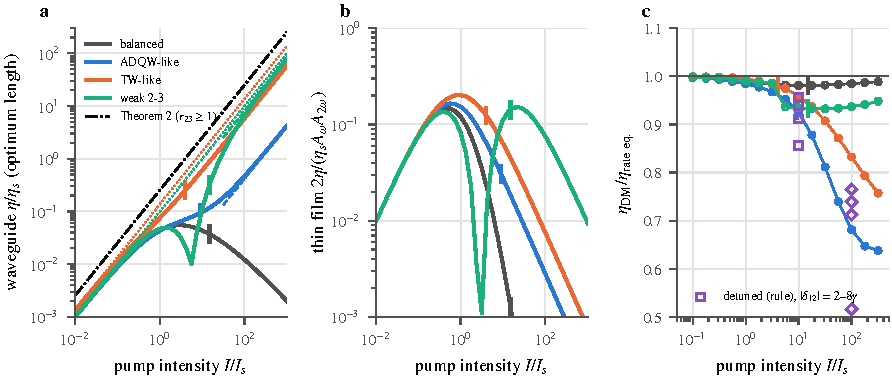
\includegraphics[width=\textwidth]{figures/fig3_saturation.pdf}
\caption{(a) Waveguide efficiency at the optimum length, in units of $\eta_s$ (Eq.~\ref{eq:etas}), against input pump intensity for four ladders (solid), with Theorem~1 (dotted), the large-intensity asymptote of Eq.~\eqref{eq:asym} (dashed) and Theorem~2 for $r_{23}\ge1$ (dash-dotted). Parameters: balanced, $r_{23}=1$, $u_0=4$, $t_{32}=t_{31}=1$; ADQW-like and TW-like, mapped from the structures of Sec.~\ref{sec:real} at $n_s=10^{11}$~cm$^{-2}$ (TW at 50~kV/cm): $r_{23}=1.65$, $u_0=4.16$, $\delta_{12}=0.22\gamma$, $\delta_{13}=0.16\gamma$, $t_{32}=1.21$, $t_{31}=0.86$, and $r_{23}=3.73$, $u_0=0.95$, $\delta_{12}=0.09\gamma$, $\delta_{13}=0.18\gamma$, $t_{32}=0.27$, $t_{31}=0.51$; weak 2--3, $r_{23}=0.3$, $u_0=4$; no background loss. Ticks mark the conservative rate-equation criterion $\hbar\Omega=|D|$ for $p_\mathrm{coh}=15$. (b) Thin film of fixed thickness, Eq.~\eqref{eq:film}, against local intensity. (c) Ratio of the efficiency from the full three-level density matrix to that of the rate-equation ladder at equal pump depletion ($\eta_s=r_{23}/4p_\mathrm{coh}$), for the four resonant ladders (circles, ticks as in a) and for the detuned ADQW-like ladder of Fig.~\ref{fig:detune}a with $|\delta_{12}|=2$--$8\gamma$ (squares, $10\Is$; diamonds, $100\Is$).}
\label{fig:sat}
\end{figure}

\section{Escaping saturation by detuning}\label{sec:detune}
Almogy and Yariv observed that detuned frequencies are preferable above saturation when the propagation length is not limited \cite{AlmogyLEOS1994}; for a symmetric ladder they found the best harmonic detuning to be about $\sqrt2$ times the pump Rabi frequency, and that detuning of opposite sign at the two frequencies, which introduces a transition-induced phase mismatch, still pays at high intensity, most of all when phase matching is imposed externally \cite[Figs.~9.7--9.9]{AlmogyThesis1995}. Vurgaftman \emph{et al.} instead detuned both transitions to the same side, so that the resonant index offsets the bulk and waveguide mismatch \cite{Vurgaftman1996SSC}. Theorem~1 makes the benefit quantitative: it is reached under saturation if the pump is detuned far enough that the transition is not saturated, $\ell_{12}I_0/\Is\lesssim1$, i.e.\ $|\delta_{12}|\gtrsim\gamma\sqrt{I_0/\Is}$, and the harmonic is detuned to restore $u=1$: $\ell_{13}=u_0\ell_{12}$, i.e.\ $|\delta_{13}|=\gamma[1/(u_0\ell_{12})-1]^{1/2}$ when $u_0\ell_{12}<1$. Choosing $\delta_{13}$ with the opposite sign to $\delta_{12}$ also detunes the 2--3 transition, $|\delta_{23}|=|\delta_{12}|+|\delta_{13}|$, which suppresses the second pump transition and extends the rate-equation regime to $I_0/\Is<p_\mathrm{coh}\min[1+\delta_{12}^2/\gamma^2,(1+\delta_{23}^2/\gamma^2)/r_{23}]$. Figure~\ref{fig:detune}a shows the result for the ADQW-like ladder. At $I_0=10\Is$ the resonant efficiency is $0.008\,I_0\eta_s/\Is$, and detuning by 6--8$\gamma$ raises it to 0.132, within 3\% of Theorem~1 and 16 times higher; at $100\Is$ the gain is 39. Because the best detuning at $10\Is$ and $100\Is$ lies at the edge of the scan, these gains are lower bounds. The cost is length, $L^*\approx(30$--$90)/A_{12}$ instead of 2--36 at resonance, so background loss matters: with $\alpha_\mathrm{bg}=10^{-2}A_{12}$ the optimum moves to $|\delta_{12}|\approx3\gamma$ and the gain at $100\Is$ falls to 32. The full density matrix (Fig.~\ref{fig:sat}c, purple) gives 0.86--0.96 of these efficiencies at $10\Is$ and 0.52--0.76 at $100\Is$. Here the rate-equation criterion is not conservative: at $\delta_{12}=-8\gamma$ and $100\Is$ the drive is at a tenth of its limit, yet the density matrix is 24\% lower. The main cause is the intensity-dependent resonant refractive index, absent from the rate-equation model, whose dispersive part grows with $\delta/\gamma$ and accumulates phase mismatch along the long detuned devices. Compensating it at the local rather than the input intensity, as a chirped or power-matched phase-matching design would, raises the ratios to 0.89--0.99 at $10\Is$ and to 0.80--0.95 at $100\Is$ for $|\delta_{12}|\ge4\gamma$ (\texttt{dm\_local.json}); for $|\delta_{12}|=2\gamma$ at $100\Is$, where $\hbar\Omega_{12}$ approaches $|D_{12}|$, it remains 0.52, a coherent effect.

\begin{figure}[t]
\centering
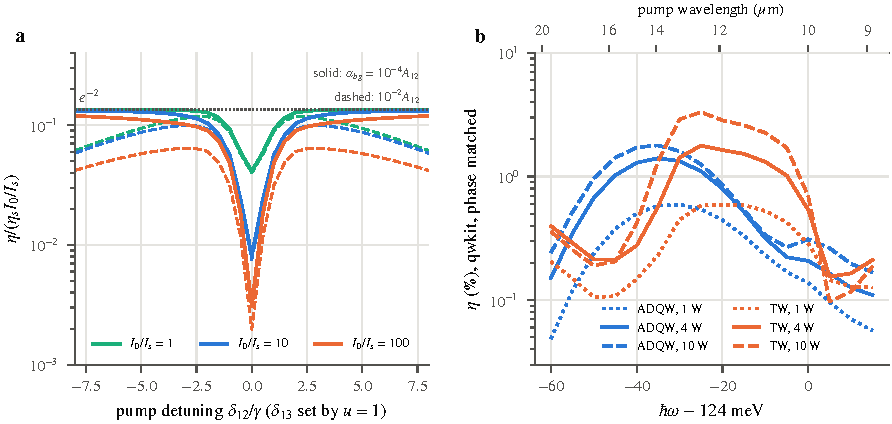
\includegraphics[width=\textwidth]{figures/fig4_detuning.pdf}
\caption{(a) Ladder model (ADQW-like, without pump depletion): efficiency per unit input intensity, in units of $\eta_s$, against pump detuning, with the harmonic detuning chosen for $u=1$ and opposite in sign, at three input intensities and two background losses. The dotted line is the Theorem~1 optimum $e^{-2}$. (b) Full qwkit simulations: phase-matched efficiency of the ADQW and the TW waveguides against pump photon energy at 1, 4 and 10~W, with the waveguide recomputed at each pump wavelength (top axis).}
\label{fig:detune}
\end{figure}

\section{Real structures}\label{sec:real}
We map two In$_{0.53}$Ga$_{0.47}$As/In$_{0.52}$Al$_{0.48}$As active regions from Ref.~\cite{OwnbyN1} onto the ladder: an ADQW (64/10/29~\AA) and a mirror-symmetric triple well (58/14/34/14/58~\AA) at 55~kV/cm, each at $n_s=5\times10^{11}$~cm$^{-2}$ per period, pumped at 10$\um$ in a 40-period InP waveguide ($\Gamma_\omega=0.39$, $\Gamma_{2\omega}=0.51$, background losses 3.3 and 0.16~cm$^{-1}$). The ladder levels are the ground state and the states with the largest resonant pump and harmonic weights; dipoles, depolarization-shifted transition energies, lifetimes (from the LO-phonon rate matrices, with all decay out of level 2 counted in $\tau_{21}$) and the modal coupling constant are taken from the full calculation. Table~\ref{tab:map} lists the parameters. The TW's pump dipole is small ($z_{12}=1.24$~nm against 1.94~nm), and its upper pump state decays in 0.56~ps, so its saturation intensity is 4.5 times higher (a factor 2.5 from the dipole and 1.8 from the lifetime) and $u_0$ is close to 1. That decay, however, leads into an intermediate state 50~meV above the ground state, which empties in 2.2~ps.

\begin{table}[t]
\centering\small
\begin{threeparttable}
\caption{Ladder parameters mapped from full qwkit calculations ($n_s=5\times10^{11}$~cm$^{-2}$, $\gamma=10$~meV, 300~K).}
\label{tab:map}
\begin{tabular}{lcc}
\toprule
 & ADQW & Triple well (55 kV/cm)\\
\midrule
$z_{12}$, $z_{13}$, $z_{23}$ (nm) & 1.94, 0.83, 2.42 & 1.24, 1.12, 2.40\\
$r_{23}$, $u_0$ (modal) & 1.56, 4.22 & 3.76, 0.94\\
$\delta_{12}/\gamma$, $\delta_{13}/\gamma$ & 0.00, 0.08 & 0.17, 0.16\\
$\tau_{21}$ (ps), $t_{32}$, $t_{31}$ & 1.02, 1.10, 0.83 & 0.56, 0.29, 0.55\\
$\Is$ (MW/cm$^2$), $P_s$ (W)\tnote{a} & 0.75, 0.43 & 3.4, 1.9\\
$\eta_s$ (Eq.~\ref{eq:etas}) & 2.5\% & 11.1\%\\
$g(u_0)$ & 0.097 & 0.135\\
Rate-equation limit, resonant pump\tnote{b} & 4.3 W & 4.4 W\\
$\eta$ at that power (qwkit) & 0.21\% & 0.55\%\\
\bottomrule
\end{tabular}
\begin{tablenotes}\footnotesize
\item[a] Pump power giving the stack-averaged intensity $\Is$.
\item[b] Power at which $\hbar\Omega_{12}=|D_{12}|$ or $\hbar\Omega_{23}=|D_{23}|$.
\end{tablenotes}
\end{threeparttable}
\end{table}

Figure~\ref{fig:real} compares phase-matched qwkit simulations from 10~mW to 300~W with the mapped ladder, Theorem~1 and the modal form of Theorem~2 (Appendix~\ref{app:modal}). For the ADQW the ladder reproduces the multilevel simulation to within 9\% up to the rate-equation limit and to within 15\% (20\% at $n_s=10^{11}$~cm$^{-2}$) up to 300~W, including the continued growth predicted by Eq.~\eqref{eq:asym}; at the lower doping the background loss ends that growth near 180~W, as discussed in Sec.~\ref{sec:sat}. At 10~mW the simulations reach 0.34 (ADQW) and 0.41 (TW) of the bound, against the ideal 0.54. For the TW the ladder overestimates the efficiency by a factor 1.3 at 10~mW, because the thermally populated intermediate state adds absorption and competing pathways that do not contribute to the ladder nonlinearity ($Q_\mathrm{eff}=0.77\,Q$, Fig.~\ref{fig:identity}c), 2.9 at the rate-equation limit and up to 7 near 30~W (4.7 at 300~W). The cause is the intermediate state: saturation parks electrons there, outside the ladder. Shortening its lifetime in the simulation from 2.2~ps to 0.80 or 0.25~ps, with detailed balance kept, raises the efficiency at 3.6~W by factors 1.5 and 1.9 (at 10~W by 1.9 and 2.9) and moves the result towards the ladder (Fig.~\ref{fig:real}b). Faster depopulation of intermediate states, for example by placing them one LO-phonon energy above a lower state with strong overlap, is therefore a design target for coupled-well active regions.

\begin{figure}[t]
\centering
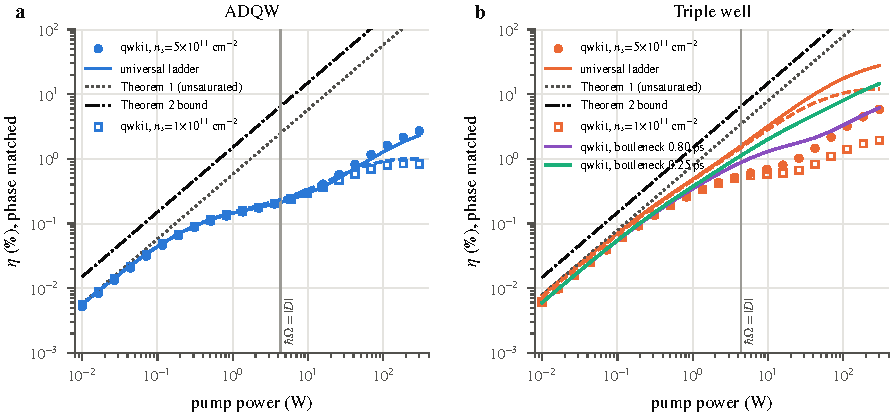
\includegraphics[width=\textwidth]{figures/fig5_qwkit.pdf}
\caption{Phase-matched efficiency against pump power from full qwkit simulations (markers) of (a) the ADQW and (b) the triple well at two doping levels, compared with the mapped ladder model (lines), Theorem~1 (dotted) and the modal bound of Theorem~2 (dash-dotted). The vertical line marks where the resonant drive leaves the rate-equation regime. In (b) the purple and green curves are qwkit simulations with the intermediate (bottleneck) state's lifetime shortened from 2.2 to 0.80 and 0.25~ps.}
\label{fig:real}
\end{figure}

Detuned pumping, the remedy of Sec.~\ref{sec:detune}, is tested in Fig.~\ref{fig:detune}b by scanning the pump photon energy in the full simulations of the same structures. The waveguide modes, confinement factors, overlap, indices and background losses are recomputed at each pump wavelength, which ranges from 8.9 to 19.4$\um$; at longer wavelengths the mode spreads ($\Gamma_\omega$ falls from 0.39 to 0.32 at 12.5$\um$ and 0.28 at 13.9$\um$) and the free-carrier and metal losses grow (to 6.2 and 7.9~cm$^{-1}$). Scanning the photon energy detunes $\delta_{12}$ and $\delta_{13}\approx2\delta_{12}$ together and so only approximates the rule, but it already gives large gains. With the pump 35~meV below resonance (13.9$\um$) the ADQW reaches 1.41\% at 4~W instead of 0.21\% (6.8 times) and 1.79\% at 10~W; with the pump 25~meV below resonance (12.5$\um$) the TW reaches 1.78\% at 4~W instead of 0.54\% (3.3 times) and 3.3\% at 10~W. At 10~mW, where saturation plays no role, the gain is 1.5 (ADQW) and 1.3 (TW), from the rise of $Q_\mathrm{eff}$ below resonance (Fig.~\ref{fig:identity}b,c) partly offset by the smaller overlap. The detuned operating points lie well inside the rate-equation criterion, whose limit rises to about 83~W for the ADQW and 39~W for the TW with the recomputed waveguide. At these operating points ($\delta_{12}=2.7$--$3.5\gamma$, 1.6--17~$\Is$) the full density matrix of Sec.~\ref{sec:sat}, applied to the mapped ladders with the recomputed waveguide, gives 0.98--1.00 of the rate-equation efficiency at 4~W and 0.87 (ADQW) and 0.99 (TW) at 10~W, so the saturable resonant index, absent from qwkit's phase-matched propagation, lowers the efficiencies by up to 13\% unless the phase matching is chirped. The resonant operating point of 10~W used in Ref.~\cite{OwnbyN1} lies beyond the 4~W limit of Table~\ref{tab:map}; the density-matrix comparison of Sec.~\ref{sec:sat} suggests that the rate-equation efficiencies there are accurate to about 15\%, but the comparisons between QPM schemes made there would be worth repeating with a detuned pump. To keep a 10$\um$ pump, the detuning would instead be built into the structure: a design that meets the detuning rule exactly needs an anharmonicity $E_{31}-2E_{21}$ of order $\pm100$~meV and should do better still.

\section{Discussion}\label{sec:disc}
\emph{Design rules.} The results reduce to six rules. (1) Rank active regions by $Q_\mathrm{eff}=|\chitwo|^2/(\aw\aww)\approx(n_\omega n_{2\omega}c^2/2\omega^2)q^2z_{23}^2/(\gamma_{12}\gamma_{13})$ and by the Rabi energy it implies at the available intensity, not by $|\chitwo|$ or by $(z_{13}z_{23}/z_{12}^2)^2$. (2) Tune the harmonic absorption to twice the pump absorption. (3) Raise the doping only until resonant absorption dominates the background loss; beyond that, doping matters at high power only through the bleached optical depth. (4) Above $\Is$, detune the pump by about $\gamma\sqrt{I/\Is}$ and the harmonic oppositely, so that $\aww\approx2\aw$. (5) Remove population bottlenecks. (6) Narrow both linewidths, which enter as $\gamma_{12}\gamma_{13}$ in the small-signal limit.

\emph{Waveguides and thin films.} Both geometries obey the same material limit: at equal local intensity Theorem~1 and Eq.~\eqref{eq:film} differ only by the geometric factors $g(u)\zeta_\omega\zeta_{2\omega}\le e^{-2}$ and $A_\omega A_{2\omega}/2\le1/2$. They differ under saturation. In a metasurface the optical depth is fixed by the stack, so the efficiency peaks near $\Is$ and then falls \cite{GomezDiaz2015}; Eq.~\eqref{eq:film} recovers that ceiling and shows that field enhancement lowers the required external intensity without raising it. Pumping an initially empty transition raises the saturation intensity \cite{Nefedkin2022} and so moves the ceiling, consistent with Eq.~\eqref{eq:film}, and a detuned film with a correspondingly larger resonant optical depth would do the same. A waveguide trades phase matching and higher pump power for an optical depth that its length supplies and that adapts to the bleaching.

\emph{Relation to prior estimates.} The textbook estimate \cite{Vurgaftman2021} is recovered as the $u\gg1$, $I_0=\Is$ limit of Theorem~1. Its generalization to detuned resonances grows without bound with pump detuning, because the saturation intensity grows; Theorem~2 and the background-loss factor $\zeta$ supply the missing limits. Numerical waveguide models that neglect saturation \cite{Chesi2023,DeLeonardis2022} are exact in the regime of Theorem~1, and the doping independence of the optimized efficiency is implicit in the observation that adding wells shortens the optimum length with little change in peak efficiency \cite{Chesi2023}. Vurgaftman \emph{et al.} solved the same rate-equation and coupled-wave model numerically, including the population-dependent resonant index, carrier heating and the waveguide modes \cite{Vurgaftman1996}. They found double resonance optimal below saturation and detuning advantageous above it, with the length held at its overall optimum; their predicted peaks, 14--16\% at 20--40~MW/cm$^2$ for InGaAs/InAlAs waveguides \cite{Vurgaftman1996} and 2.6\% in a later design \cite{VurgaftmanNLO1996}, rely on dipole ratios $z_{23}/z_{12}\approx3.2$ from an eight-band calculation. For their 64.5/18/36.5~\AA\ structure, our one-band model reproduces the transition energies to within 3~meV but gives $z_{23}/z_{12}=1.1$; the Thomas--Reiche--Kuhn sum rule allows a ratio of 3.2 only if $z_{12}\le0.8$~nm. Since the efficiency scales as $(z_{13}z_{23}/z_{12}^2)^2$, such predictions are sensitive to the band model, and at their operating point the 2--3 transition is driven at $\hbar\Omega_{23}\approx1.1$--$2.9\,|D_{23}|$ (for $z_{12}=0.8$--1.5~nm; \texttt{vurg\_check.json}), beyond the regime where the population-dependent susceptibility used there and here is reliable. Almogy and Yariv obtained the symmetric-ladder case of Theorem~1, a length-limited bound on the harmonic intensity, and the numerical observation that a resonant waveguide has no intensity ceiling when its length is optimized, and used non-perturbative rotating-wave susceptibilities to follow how the perturbative conclusions change at saturating intensity \cite{Almogy1994,AlmogyLEOS1994,Almogy1995JNOPM,AlmogyThesis1995}. Evaluated over a fixed length, such as one absorption length, their efficiencies do show a ceiling, as Eq.~\eqref{eq:lbound} requires. The identity, Theorem~2, the closed-form slope with its ceiling condition, the detuning rule and the generalized length bound extend their results to arbitrary ladders and phase-matching patterns. Our density-matrix check reproduces their closed-form saturated susceptibility and supports the rate-equation results to within 36\% up to $300\Is$ for resonant pumping, and for detuned pumping once the saturable index is compensated. That resonant index, which Almogy \emph{et al.} identified as a possible dominant limitation on conversion \cite{AlmogyOL1994PM,AlmogyThesis1995}, is indeed the main correction we find for detuned operation.

\emph{Limitations.} The identity of Eq.~\eqref{eq:identity} relies on Lorentzian lines; inhomogeneous broadening changes the off-resonant ratio of $\chitwo$ to absorption and therefore $Q_\mathrm{eff}$ under detuning. The theorems assume the rate-equation regime, no population inversion, the energy-conserving coupling of Eq.~\eqref{eq:cm} (in a resonant absorbing medium $\chi^{(2)}(\omega;2\omega,-\omega)$ need not equal $\chitwo{}^*$, which matters only when pump depletion by the harmonic is significant; the density-matrix calculation, which computes the pump polarization self-consistently, stays below the rate-equation results and the bound in every case examined) and, for the plane-wave form, uniform intensity; the modal form (Appendix~\ref{app:modal}) evaluates Eq.~\eqref{eq:t2} at the peak intensity in the active region. The dipoles of the real structures come from a one-band model; the comparison with Ref.~\cite{Vurgaftman1996} above suggests that multiband checks of $z_{23}/z_{12}$ are worthwhile. The density-matrix check uses the rotating-wave approximation and steady state, and, being three-level, cannot capture coherent mixing with other subbands at large Rabi energies (in the TW the transition from the intermediate state to level 4 lies 9.4~meV above $2\hbar\omega$). In the qwkit simulations the depolarization and Hartree shifts are frozen at their equilibrium values under saturation; the depolarization shifts of the ladder transitions are at most 3.0~meV (ADQW) and 1.8~meV (TW), and recomputing both shifts self-consistently with equal ladder populations, the large-intensity limit, moves the ladder transitions by at most 2.4~meV (ADQW) and 2.2~meV (TW), i.e.\ by less than $0.25\gamma$. Thermal limits are not included: the intensities discussed are pulsed-regime intensities. The extension to difference-frequency generation and the design of structures that meet the detuning rule exactly at a fixed pump wavelength are natural next steps.

\section{Conclusion}
The efficiency of resonant ISB second-harmonic generation is governed by the Rabi energy of the pump on the 2--3 transition in units of the linewidths. The identity $|\chitwo|^2=Q\aw\aww$ makes the optimum-length efficiency independent of doping, of the pump and harmonic dipoles and of detuning, with the maximum $e^{-2}(\hbar\Omega_{23})^2/4\gamma_{12}\gamma_{13}$ at $\aww=2\aw$. A rigorous bound, only $e^2/4\approx1.85$ times larger when the 2--3 term dominates, holds for any saturation state, length and phase-matching scheme. Under saturation a waveguide keeps gaining with pump intensity, as confirmed by the full density matrix, while a thin film of fixed optical depth saturates; detuning restores the unsaturated limit. For In$_{0.53}$Ga$_{0.47}$As/In$_{0.52}$Al$_{0.48}$As structures, full simulations give phase-matched efficiencies of 1.4--1.8\% at 4~W with the pump tuned below resonance, 3--7 times the resonant values, and identify a population bottleneck that structure design can remove.

\appendix
\section{Proof of Theorem 2}\label{app:proof}
\emph{Pointwise inequality.} With $a,b\ge0$, $|a/D_{12}-b/D_{23}|\le a/|D_{12}|+b/|D_{23}|$. Write the right side as the scalar product of $(z_{12}\sqrt{a\gamma_{12}}/|D_{12}|,\ z_{23}\sqrt{b\gamma_{23}}/|D_{23}|)$ and $(z_{23}\sqrt{a/\gamma_{12}},\ z_{12}\sqrt{b/\gamma_{23}})$, after multiplying by $z_{12}z_{23}$. Cauchy--Schwarz gives $z_{12}^2z_{23}^2|a/D_{12}-b/D_{23}|^2\le(z_{12}^2a\gamma_{12}/|D_{12}|^2+z_{23}^2b\gamma_{23}/|D_{23}|^2)(z_{23}^2a/\gamma_{12}+z_{12}^2b/\gamma_{23})$. The first factor is $\aw n_\omega c\varepsilon_0/(N\omega q^2)$, and $z_{13}^2(a+b)\gamma_{13}/|D_{13}|^2=\aww n_{2\omega}c\varepsilon_0/(2N\omega q^2)$; Eq.~\eqref{eq:cs} follows. Equality holds for $b=0$.

\emph{Propagation.} Equation~\eqref{eq:cm} gives $E_2(L)=\int_0^L(i\omega/n_{2\omega}c)s\chitwo E_1^2e^{i\Delta kx}w\,dx$ exactly, whatever the depletion of $E_1$. With $|s|\le1$ and $|E_1|^2=I_1/(2n_\omega\varepsilon_0c)$,
$|E_2(L)|\le(\omega/n_{2\omega}c)(2n_\omega\varepsilon_0c)^{-1}\int|\chitwo|I_1w\,dx$. Insert $|\chitwo|\le(Q\aw\aww)^{1/2}\le(\sup Q\,\hat\zeta_\omega\hat\zeta_{2\omega}\,\alpha_{1,t}\alpha_{2,t})^{1/2}$ and apply Cauchy--Schwarz: $\int(\alpha_{1,t}I_1^2)^{1/2}(\alpha_{2,t}w^2)^{1/2}dx\le[\int\alpha_{1,t}I_1^2dx]^{1/2}[\int\alpha_{2,t}w^2dx]^{1/2}$. The second integral is $1-w(0)^2\le1$ since $d(w^2)/dx=\alpha_{2,t}w^2$. For the first, energy conservation in Eq.~\eqref{eq:cm} gives $d(I_1+I_2)/dx=-\alpha_{1,t}I_1-\alpha_{2,t}I_2\le-\alpha_{1,t}I_1$, so with $J=I_1+I_2\le I_0$ and $I_1\le J$, $\int\alpha_{1,t}I_1^2dx\le\int\alpha_{1,t}I_1J\,dx\le-\int J\,dJ\le I_0^2/2$. Collecting factors, $I_2(L)/I_0\le(\kappa^2I_0/2)\sup Q\,\hat\zeta_\omega\hat\zeta_{2\omega}$, and the maximum of $Q(\rho)$ over $a/(a+b)$ gives the right side of Eq.~\eqref{eq:t2}.

\section{Large-intensity asymptote}\label{app:asym}
In units $\tilde x=A_{12}x$, $p=I_1/\Is$, and with the pump phase fixed, the harmonic amplitude $e_2$ (normalized so $|e_2|^2=I_2/\Is$) obeys $de_2/d\tilde x=ic\,C_\infty-[m_\infty/2p(\tilde x)]e_2$ with $p(\tilde x)=p_0-k_\infty\tilde x$ and $|c|^2=\eta_s/u_0$. Changing variable to $p$, $e_2(p_L)=(icC_\infty/k_\infty)\int_{p_L}^{p_0}(p_L/p)^\nu dp=(icC_\infty/k_\infty)\,p_0\,(y^\nu-y)/(1-\nu)$ with $y=p_L/p_0$. The maximum over $y$ is at $y^*=\nu^{1/(1-\nu)}$ and equals $p_0\nu^{\nu/(1-\nu)}$, which gives Eq.~\eqref{eq:asym}. The optimum is reached while the pump is still strong ($y^*=0.13$--$0.32$ for the ladders of Fig.~\ref{fig:sat}), so the regions of weak saturation near the end of the device do not contribute.

\section{Modal form}\label{app:modal}
In a waveguide with normalized TM profiles $f_j(z)$, confinement factors $\Gamma_j$ and nonlinear overlap $O=|\int_\mathrm{QW}f_1^2f_2^*dz|^2/w$, the modal coupled-mode equations have $K^2=\omega^2O/(2n_\omega^2n_{2\omega}\varepsilon_0c^3)$ and modal losses $\Gamma_j\alpha_j+\alpha_{\mathrm{bg},j}$ \cite{OwnbyN1}. The proof of Appendix~\ref{app:proof} then gives $\eta\le K^2\sup Q\,P_0/(2\Gamma_\omega\Gamma_{2\omega})$ (used in Fig.~\ref{fig:real}). By Cauchy--Schwarz, $O\le\max_\mathrm{QW}|f_1|^2\,\Gamma_\omega\Gamma_{2\omega}/w$, so this equals the plane-wave bound of Eq.~\eqref{eq:t2} evaluated at an intensity no larger than the peak pump intensity in the active region; it reaches that value only if $f_1$ and $f_2$ are uniform over the stack.

\bibliographystyle{unsrtnat}
\bibliography{refs}
\end{document}
